\subsection{Fuerza Magnética}
\begin{tikzpicture}
        \draw [->] (0,0) -- (0,2) node[left = 1]{\(\vec{F_m}\)};
        \draw [->](0,0) -- (2,0) node[above = 1]{\(\vec{B}\)};
        \draw [->] (0,0,0) -- (1.7,0,1.5) node[above = -20]{\(\vec{v}\)};
\end{tikzpicture}
\newline
\noindent La fuerza magnética actua sobre las cargas en movimiento y se define, para una carga en movimiento como:
\[
        \boxed{\vec{F_m} = q\hspace{2mm} \vec{v} \times \vec{B}}
\]
\noindent \(\bm{\vec{F_m}}\) es perpendicular \(\bm{\perp}\) a \(\bm{\vec{B}}\) y a \(\bm{\vec{v}}\) y siempre irá en el sentido que indique la carga, la velocidad y el campo, por lo que la Fuerza magnética es proporcional a la carga, el campo y a la velocidad.
\\
Algunas propiedades que nos vendrán bien a la hora de calcular son las siguientes, respecto al producto vectorial:
\begin{enumerate}
        \item \(\bm{\hat{\imath} \times \hat{\imath} = 0}\) Y lo mismo ocurre para cualquier otra combinación.
        \item \(\bm{\hat{\imath}\times \hat{\jmath} = \hat{k}}\), \(\bm{\hat{\jmath}\times\hat{k}=\hat{\imath}}\),\(\bm{\hat{\imath}\times\hat{k}=\hat{\jmath}}\).
        \item \(\bm{\vec{v} \times \vec{B} = - \vec{B} \times \vec{v}}\)
        \item El modulo es \(\bm{\left | \vec{v} \right |\left | \vec{B} \right |\sin{\alpha}}\).
        \item La dirección, es la perpendicular entre \(\vec{v}\) y\(\vec{B}\).
        \item El sentido viene indicado por la regla de la mano derecha.
\end{enumerate}
\noindent Además consideraremos \(\bm{\bigotimes}\) para cuando el campo vaya hacia dentro del papel y \(\bm{\bigodot}\) cuando sea hacia fuera.
\subsubsection{Conservación de la Energía, Trabajo y Movimiento}
\noindent La Fuerza Magnética no es una fuerza conservativa por lo que la energía requerida para mover un cuerpo, en un caso inicial, una carga entre dos puntos, depende de su trayectoria.
\[
        W_{1 \rightarrow 2}= \int^2_1\vec{F}\hspace{2mm}\mathrm{d}\vec{r} \hspace{1mm}=\hspace{1mm} q\int^2_1\vec{v}\times\vec{B}\hspace{2mm}\mathrm{d}\vec{r}\hspace{1mm}=\hspace{1mm}0 \textnormal{J}
\]
\noindent De esta expresión podemos sacar varias conclusiones:
\begin{itemize}
        \item Al ser el trabajo nulo, \(\bm{\Delta E_c = 0} \hspace{2mm}\bm{\Rightarrow}\hspace{2mm}\bm{\vec{v}=cte} \hspace{2mm}\bm{\textnormal{\&}}\hspace{2mm} \bm{\vec{v}\times\vec{B}\perp\mathrm{d}\vec{r}}\)
        \item Por esta misma razón la fuerza no puede ser nula, por lo que la aceleración tampoco y por ende, la velocidad tampoco \(\bm{\vec{F}\not =0 \Rightarrow\vec{a}\not=0\Rightarrow\frac{\mathrm{d}\vec{v}}{\mathrm{d}t} \not=0}\).
        \item \(\bm{\vec{F_m} = \vec{F_\tau}+\vec{F_n}}\) La fuerza magnética es la suma de sus componentes normal \(\bm{\vec{F_n}}\) y tangencial \(\bm{\vec{F_\tau}}\).
        \item El movimiento de un cuerpo afectado por el \(\bm{\vec{B}}\) es variable y complejo, por eso solo estudiamos casos específicos, por ejemplo en el caso de un Helicoidal, el campo tiene una forma de cuello de botella y no lo estudiaremos, pero el resto, en casi todos los casos que veremos, se moverán a favor de \(\bm{\vec{B}}\).
\end{itemize}
\noindent Si consideramos solamente la fuerza tangencial \(\bm{\vec{F_{\tau}}=0}\) podemos obtener una expresión con la cual calcular la velocidad con la que gira la particula y el radio de la circunferencia con la que gira:
\[
        \vec{F_m} = \vec{F_n}
\]
\[
        q\hspace{2mm} \vec{v} \times \vec{B} \hspace{1mm} = \hspace{1mm} m\vec{a}
\]
\[
        q\left | \vec{v} \right |\left | \vec{B} \right |\sin{\alpha} \hspace{1mm} = \hspace{1mm} m\frac{\left | \vec{v} \right |^2}{R}
\]
\[
        \boxed{v = \frac{qBR}{m}\sin{\alpha}}
\]
Siendo \(\bm{R}\) el radio de la circunferencia y \(\bm{\vec{v}}\) la velocidad normal.
\subsection{Ley de Lorentz}
\noindent Esta es una expresión bastante simple que relaciona la fuerza magnética y la electrostática:
\[
        \boxed{\bm{\vec{F_T} =\vec{F_m} + \vec{F_e} =q(\vec{E} + \vec{v}\times\vec{B})}}
\]
\subsubsection{Selector de Velocidades}
\begin{wrapfigure}{r}{4cm}
        \begin{tikzpicture}
                \draw [] (0,0) -- (4,0) node[above = 1]{\(\bm{+}\)};
                \draw [] (0,-2) -- (4,-2)node[above = -20]{\(\bm{-}\)};
                \draw [->] (0,-.5) -- (.75,-.5) node[above = 1]{\(\vec{v}\)};
                \draw [->] (1,0) -- (1,-1.75) node[right = 1]{\(\vec{B}\)};
                \draw [->] (0.3,-1) -- (0.3,-1.7) node[right = 1]{\(\vec{F_e}\)};
        \end{tikzpicture}
\end{wrapfigure}
\noindent Este es un caso muy particular para aplicar la Ley de Lorentz. Al tener un espacio donde actúan la fuerza magnética y la eléctrica, e introducimos una carga con cierta velocidad podemos concluir en lo siguiente:
\[
        \vec{F_{\tau}}=0
\]
\[
        \boxed{\vec{F_m} = -\vec{F_e}}
\]
Son la misma fuerza, pero en sentidos opuestos
\subsection{Fuerza Magnética en un hilo conductor}
\[
        \boxed{\vec{F_m} = I \hspace{2mm}\vec{l}\times\vec{B}}
\]
No nos interesa saber como llegar a esta expresión, ya que hay que trabajar con la Densidad de Carga y la definición de Intensidad, por lo que no se explicará, en un principio en este documento.
\subsection{Espira}
\noindent Si consideramos una espira rectangular, con un \(\bm{\vec{B}\perp\vec{S}}\) de la espira, y hacia dentro \(\bm{\bigotimes}\) la Fuerza magnética será la misma en aquellos lados con la misma longitud.
\\
Con esta premisa, podemos ser capaces de calcular el \underline{momento magnético} que nos indica la fuerza necesaria para mantener en equilibrio, o desplazar la espira de un punto en equilibrio a uno inestable.
\[
        \vec{M} \hspace{1mm} = \hspace{1mm} \vec{m}\times\vec{B} \hspace{1mm} = \hspace{1mm} \boxed{IN \hspace{2mm} \vec{S} \times \vec{B}}
\]
Esta expresión nos dice dos cosas, la primera y más importante es que el momento está afectado por la orientación del campo y el de la superficie de la espira. Para que estén en equilibrio, el campo y la superficie deben de ser \textbf{paralelos} entre si, no \textbf{antiparalelos}, es decir, que aunque el ángulo entre ambos sea cero, tienen sentidos opuestos.
\\
La segunda, es que el sentido de la corriente, y por ende la dirección del vector superficie \(\bm{\vec{S}}\) va en función de la corriente, aplicando la regla de la mano derecha. %TODO Añadir un esquema de la espira%
\subsection{Ley de Biot y Savart}
\noindent Si consideramos un conductor, indefinidamente largo y sin una forma definida, por el que circula corriente, definitivamente podemos calcular el campo magnético de la figura en cualquier punto de esta:
\[
        \boxed{\vec{B}(P) \hspace{1mm}= \hspace{1mm}\int_{S} I\hspace{1mm}\frac{\mathrm{d}\vec{l}\times\vec{r}}{\left | \vec{r} \right |^3}\hspace{2mm}\frac{\mu_{\textnormal{o}}}{4\pi} \hspace{5mm}\textnormal{\textbf{[T]}}}
\]
\noindent Podemos observar que esta integral, puede llegar a ser muy complicada de calcular, y solo se recurrirá a ella en casos de extrema simetría.\\
El campo magnétostático se mide en Teslas \textbf{T}, que equivalen a \(\mathbf{10^4}\) Gauss, \textbf{G}.
\subsubsection{Espira Circular}
\begin{wrapfigure}{r}{4cm}
        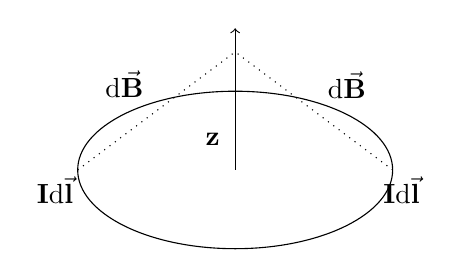
\begin{tikzpicture}
                \draw (0,0) ellipse (2cm and 1cm);
                \draw[ dotted] (2,0) -- (0,1.5) node[above = -12, right= 30] {\(\mathbf{\mathrm{d}\vec{B}}\)} node[ above = -50, right=50] {\(\mathbf{I\mathrm{d}\vec{l}}\)};
                \draw[dotted] (-2,0) -- (0,1.5) node[left = 40, above = -20] {\(\mathbf{\mathrm{d}\vec{B}}\)} node[ above = -50, left=55] {\(\mathbf{I\mathrm{d}\vec{l}}\)};
                \draw[->] (0,0) -- (0,1.8) node[above = -40, left= 2] {\textbf{z}};
        \end{tikzpicture}
\end{wrapfigure}
\noindent Este es un caso muy específico donde veremos el cálculo del campo magnetostático usando la \underline{Ley de Biot y Savart}
\[
        \mathrm{d}\vec{B_z}\hspace{1mm}=\hspace{1mm}\left | \mathrm{d}B \right |\cos{\alpha}\hspace{1mm}\hat{k} \hspace{1mm}=\hspace{1mm} I\hspace{1mm}\sin{\frac{\pi}{2}}\hspace{2mm}\frac{\mu_{\textnormal{o}}}{4\pi} \frac{\left | R \right  |r}{R^{3/2}R}\hspace{1mm}=\hspace{1mm}\frac{\mu_{\textnormal{o}}rI\mathrm{d}l}{4\pi(r^2+z^2)^{3/2}}
\]
\noindent Siendo \(\mathbf{R}\) el diametro de la espira, \(\mathbf{r}\) el radio de la espira y \(\mathbf{z}\) la altura del punto a calcular.
\[
        \boxed{B_z \hspace{1mm} = \hspace{1mm}\int \hspace{1mm} \mathrm{d}B_z = \frac{Ir^2\mu_{\textnormal{o}}}{2(r^2+z^2)^{3/2}}}
\]
\subsection{Ley de Ampere}
\noindent Esta ley es otra de las formas para calcular el campo magnetostático de un cuerpo, sabiendo que el campo es siempre circular, y está encerrado en líneas cerradas, podemos deducir que:
\[
        \boxed{\oint \vec{B}\mathrm{d}\vec{l} = I\mu_{\textnormal{o}}} \hspace{.5cm} \propto \hspace{.5cm} \oint \vec{E}\mathrm{d}\vec{S} = \frac{Q_\textnormal{int}}{\epsilon_o}
\]
\noindent Podemos observar que la Ley de Gauss es la "equivalente" a la Ley de Ampere.
\subsubsection{Solenoide}
\noindent El campo entra y sale del solenoide, por lo que habrá unos puntos con un campo magnético entrante y otro saliente, el resto se anularan:
\[
        \boxed{B \hspace{1mm}=\hspace{1mm} \frac{\mu_{\textnormal{o}}IN}{l}\hspace{2mm}\Rightarrow \hspace{2mm}\vec{B}\hspace{1mm}=\hspace{1mm}\mu_\textnormal{o}In \hspace{1.5mm}\hat{n}}\]
Siendo \(\mathbf{l}\) la longitud del solenoide. y \(\mathbf{n}\) el cociente entre el número de espiras y la longitud \(\mathbf{N/l}\).
\subsection{Fuerza entre dos hilos infinitamente largos y paralelos}
El sentido del campo va en función de como circule la corriente, si la corriente se mueve hacia arriba, el sentido será antihorario, y viceversa.
\[
        \boxed{F_{1\rightarrow 2} \hspace{1mm} = \hspace{1mm} I_2\vec{l_2} \times\vec{B_1}}
\]
\noindent Aquí calculamos la fuerza magnética que se genera en el conductor 2 por el conductor 1.
\[
        \boxed{F_{2\rightarrow 1} \hspace{1mm} = \hspace{1mm} I_1\vec{l_1} \times\vec{B_2}}
\]
\noindent Aquí calculamos la fuerza magnética que se genera en el conductor 1 por el conductor 2.
\[
        \boxed{B_n \hspace{1mm} = \hspace{1mm}\hat{l_n}\times\hat{R}\hspace{2mm}\frac{\mu_{\textnormal{o}}I_n}{2\pi d}}
\]
\noindent Podemos ver que \(\mathbf{\hat{R}}\) es la distancia al punto, como un vector unitario y \(\mathbf{\hat{l_n}}\) será el sentido del cable.